\documentclass[a4paper,utf8]{article}
\usepackage{exemple}
\usepackage[normalem]{ulem}
\usepackage{amsfonts}
\usepackage{graphicx}
\usepackage{MnSymbol,wasysym}
\usepackage{hyperref}
\usepackage[french]{babel}
\usepackage{graphicx}

\formation{L3MI}
\date{15/01/2017}
\matiere{Conception Orient�e Objet}
\titre{Projet : Tetris Attck }

\newcommand\code[1]{\textsf{#1}}
\newcommand\srdjan[1]{{\color{red} #1}}

\begin{document}

\entete

\begin{center}
	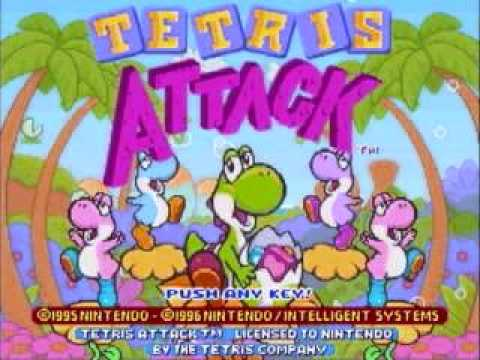
\includegraphics[scale=0.9]{img1.jpg}
\end{center}

\section{Description du Projet}
Tetris Attack est un puzzle-game � 2 joueurs sorti en 1995 sur Super Nintendo. Ce jeu est une variante du bien connu Tetris � 2 joueurs. Dans cette version, l'objectif est d'assembler des blocs entre eux afin de les faire disparaitre avant que l'ensemble des blocs n'atteignent le haut de l'ecran. Toutefois, ici, 2 joueurs s'affrontent en parallele et peuvent � l'aide de diff�rentes combinaisons envoyer de nouveaux blocs de briques � leur adversaire afin de pr�cipiter sa perte. Ce jeu couple � la fois, la simplicit� de Tetris � la dynamicit� n�cessaire d'un bon Versus.

\section{L'Organisation }

\subsection{L'Equipe}
\begin{itemize}
\item vincent : jeu principal , graphique , ia 
\item loick : jeu principal , graphique , ia 
\item mohammed: menu , diff�rent ecrans pour config , graphique
\item kevin: menu , diff�rent ecrans pour config , graphique
\end{itemize}

\subsection{Le Travail r�aliser}
A l'heure actuel le menu touche a sa fin principalement fait par loick qui a r�liser toutes les animations : ecran titre, curseur , ecran de fond ainsi que les panels .
Pour ma part (vincent) j'ai realise la selection des personnages pour 1 et 2 joueurs et une grille un joueur fonctionnelle ainsi que l'incorporation des sons dans le jeu.
Du cote de Kevin il travaille toujours avec mohammed sur la modification des commandes qui traine malgre mes relances toutes les semaines.

\end{document}